\newpage
\chapter*{Введение}
\addcontentsline{toc}{chapter}{Введение}
С момента зарождения в конце \Rmnum{20} века идея квантовых вычислений
пленит умы ученых, занимающихся различными областями
науки$[\ref{lit:nil-chang}, \ref{lit:valiev-kokin}, \ref{lit:valiev}]$. С
развитием технологий задача построения квантового компьютера
становится все более реальной. Успешные эксперименты по реализации
квантовых алгоритмов на малом числе кубитов$[\ref{lit:nv-deutsch}]$ демонстрируют прогресс в
этой области.

    Основным элементом квантового компьютера является кубит(квантовый бит)
-- двухуровневая система, которой можно эффективно управлять. К кубиту
предъявляют немколько требований:
\begin{enumerate}
\itemВысокая дискретность энергетического спектра, озволяющая четко
  разделять логические состояния |0> и |1>.
\itemСуществование механизмов инициализации, управления и измерения
  состояний кубита
\itemБольшие времена релаксации и дефазировки логических состояний
\end{enumerate}

Большинство квантовых алгоритмов требуют также контроля взаимодействия
двух произвольных кубитов. Полноценным, полезным квантовым компьютером
можно будет считать систему, насчитывающую порядка нескольких тысяч
кубитов. На сегодняшний день самыми перспективными
видятся разработки в области твердотельных структур. Наиболее
популярные из них:
\begin{enumerate}
\itemСверхпроводниковые элементы$[\ref{lit:tsukanov-super-cond-one}, \ref{lit:tsukanov-super-cond-two}]$
\itemКвантовые точки$[\ref{lit:dots}]$
\itemИмплантированные атомы$[\ref{lit:implant}]$
\itemИоны в ловушках$[\ref{lit:ion-trap}]$
\end{enumerate}

Основная проблема всех перечисленных систем в том, что для
удовлетворения вышеописанным требованиям они должны находится при
очень низких температурах (<100мК), когда энергия размерного
квантования системы много больше энергии тепловых флуктуаций. Такие
жесткие условия накладывают сильные ограничения на дизайн
кубита. Возникает желание смягчить это ограничение. Для этого
требуется система, способная долго сохранять когерентность при высоких
температурах (желательно -- комнатных). На сегодняшний день известно
только две таких системы. Первая из них, раствор молекул некоторых
органических веществ (например, раствор ацетона в хлороформе),
представляет собой объект, на котором в 1998 году были
продемонстрированы принципы квантовых вычислений$[\ref{lit:first-demonstration}]$. Однако
максимальное возможное количество кубитов -- ядерных спинов атомов
водорода, углерода и др., входящих в структуру молекулы, ограничено
числом атомов в молекуле. Вторая такая система есть дефект
кристаллической решетки алмаза, образованный соседними атомом азота(N)
и вакансией(V). Принятое обозначение такого дефекта -- NV -- указывает
на структурный состав, а название -- ``NV-центр'' -- говорит о том,
что он представляет собой так называемый центр окраски по отношению к
чистому алмазному субстрату. Схематическое изображение NV-центра
показано на рисунке (\ref{fig:nv}). Данная твердотельная система дает ряд
преимуществ: длительное сохранение когерентности при комнатных
температурах, возможность быстрой инициализации и быстрого измерения
состояния кубита ($\sim$10нс)$[\ref{lit:lumin-collins}, \ref{lit:lumin-Hanzawa}]$, возможность создания упорядоченных
двумерных массивов, содержащих произвольное количество одиночных
NV-центров, что гарантирует возможность масштабирования. Общепринятым
способом выбора базисных состояний кубита на NV-центре |0> и |1> считается выбор уровней энергии
соответствующих проекциям спина m=0 и одной из проекций m=1 или m=-1. Несмотря на
сравнительно высокие скорости выполнения однокубитных операций в
NV-центре, для эффективной работы полномасштабного квантового
компьютера их не достатачно. Исследования сверхбыстрых (1-2нс) спиновых
вращений производились в нескольких работах$[\ref{lit:gigahertz}, \ref{lit:excitef-oscilations}]$, однако этот вопрос
все еще слабо исследован.
\begin{figure}[h!]\centering
  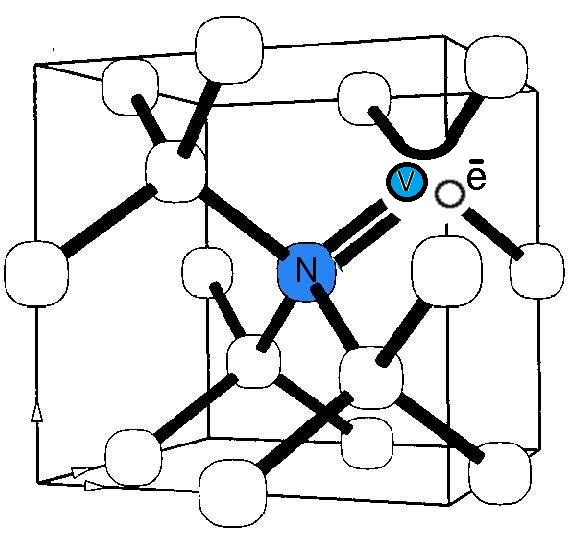
\includegraphics[width=1\textwidth]{nv}
  \caption{Схема NV-центра в алмазе.}\label{fig:nv}
\end{figure}

\section*{Цель работы}
Целью данной работы явлется исследование одного из методов быстрого ($\sim$1нс)
вращения спина: использование микроволного поля большой амплитуды. За
основу исследования взята работа $[\ref{lit:gigahertz}]$. Производя варьирование формы мощного и короткого
магнитного импульса, были сделаны попытки отыскать оптимальную. В
первой части работы было произведено аналитическое решение задачи в
двухуровневом приближении. Во второй части произведено численное
решение трехуровневой задачи при различных формах микроволнового
импульса, произведено сравнение результатов с аналитическими и
экспериментальными результатами, полученными в работе
$[\ref{lit:gigahertz}]$.
\section*{Постановка задачи}
Имеется одиночный NV-центр (отрицательно заряженная форма). Кубит,
кодирующийся суперпозицией электронных спиновых состояний центра с
$m_s$=$0$ и $m_s$=$-1$, долго сохраняет когерентность при комнатной
температуре, характеризуется высокой частотой однокубитных вращений,
обеспечивает быструю инициализацию и измерение конечного состояния.

Наложение постоянного магнитного поля приводят к снятию вырождения с
уровней $m_s$=$1$ и $m_s$=$-1$, что позволяет селективно возбуждать один из
переходов |$0$> -> |$1$> или |$0$> -> |$-1$> с частотами
$\omega_{\pm}$. Для этого частота переменного поля должна быть близка к
частоте выбранного перехода. Амплитуда переменного поля является
медленно меняющейся со временем функцией.
\begin{enumerate}
\itemИспользуя приближение вращающейся волны, аналитически редуцировать
трехуровневую задачу к двухуровневой, ограничившись рассмотрением
резонансного перехода |$0$> -> |$-1$>.
\itemПровести численное моделирование трехуровневой динамики электронного
спина NV-центра.
\itemПровести оптимизацию однокубитных вращений на примере перехода
|$0$> -> |$-1$>, варьируя форму и амплитуду огибающей резонансного
 импульса. Сравнить результаты с результатами работы [\ref{lit:gigahertz}].
\end{enumerate}

